SSD网络主体设计的思想是特征分层提取,并依次进行边框回归和分类。因为不同层次的特征图能代表不同层次的语义信息,低层次的特征图能代表低层语义信息(含有更多的细节),能提高语义分割质量,适合小尺度目标的学习。高层次的特征图能代表高层语义信息,能光滑分割结果,适合对大尺度的目标进行深入学习。所以作者提出的SSD的网络理论上能适合不同尺度的目标检测。

所以SSD网络中分为了6个stage,每个stage能学习到一个特征图,然后进行边框回归和分类。SSD网络以VGG16的前5层卷积网络作为第1个stage,然后将VGG16中的fc6和fc7两个全连接层转化为两个卷积层Conv6和Conv7作为网络的第2、第3个stage。接着在此基础上,SSD网络继续增加了Conv8、Conv9、Conv10和Conv11四层网络,用来提取更高层次的语义信息。如下图3.1所示就是SSD的网络结构。在每个stage操作中,网络包含了多个卷积层操作,每个卷积层操作基本上都是小卷积。
\begin{uscfigure}
	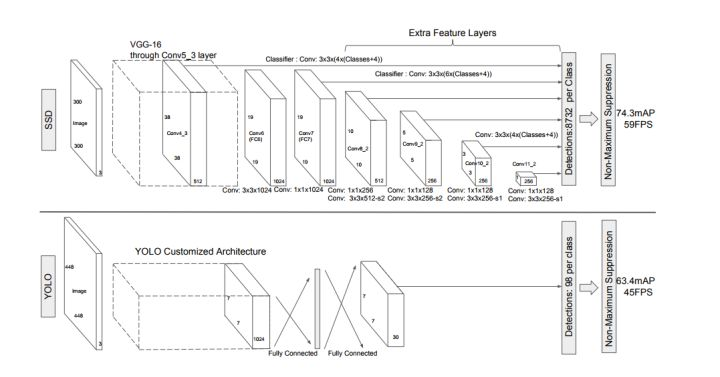
\includegraphics[width=\textwidth]{./Pictures/ssd_modual.jpg}
	\caption{RCNN}
\end{uscfigure}
骨干网络:SSD前面的骨干网络选用的VGG16的基础网络结构,如上图所示,虚线框内的是VGG16的前5层网络。然后后面的Conv6和Conv7是将VGG16的后两层全连接层网络(fc6, fc7)转换而来。另外:在此基础上,SSD网络继续增加了Conv8和Conv9、Conv10和Conv11四层网络。图中所示,立方体的长高表示特征图的大小,厚度表示是channel。

